
\documentclass{exam}

\usepackage{graphicx}
\usepackage[fleqn]{amsmath}
\usepackage{unitsdef} 
\usepackage{cancel}
\usepackage{float}
\usepackage{mdwlist}
\usepackage{booktabs}
\usepackage{cancel}
\usepackage{polynom}
\usepackage{caption}
\usepackage{fullpage}
\usepackage{enumerate}
\usepackage{parskip}

% \newcommand{\degree}{\ensuremath{^\circ}} 
\everymath{\displaystyle}

\newunit{\inch}{in}
\newunit{\foot}{ft}
\newunit{\cemtimeter}{cm}

% \begin{figure}[H]
%   \centering
%   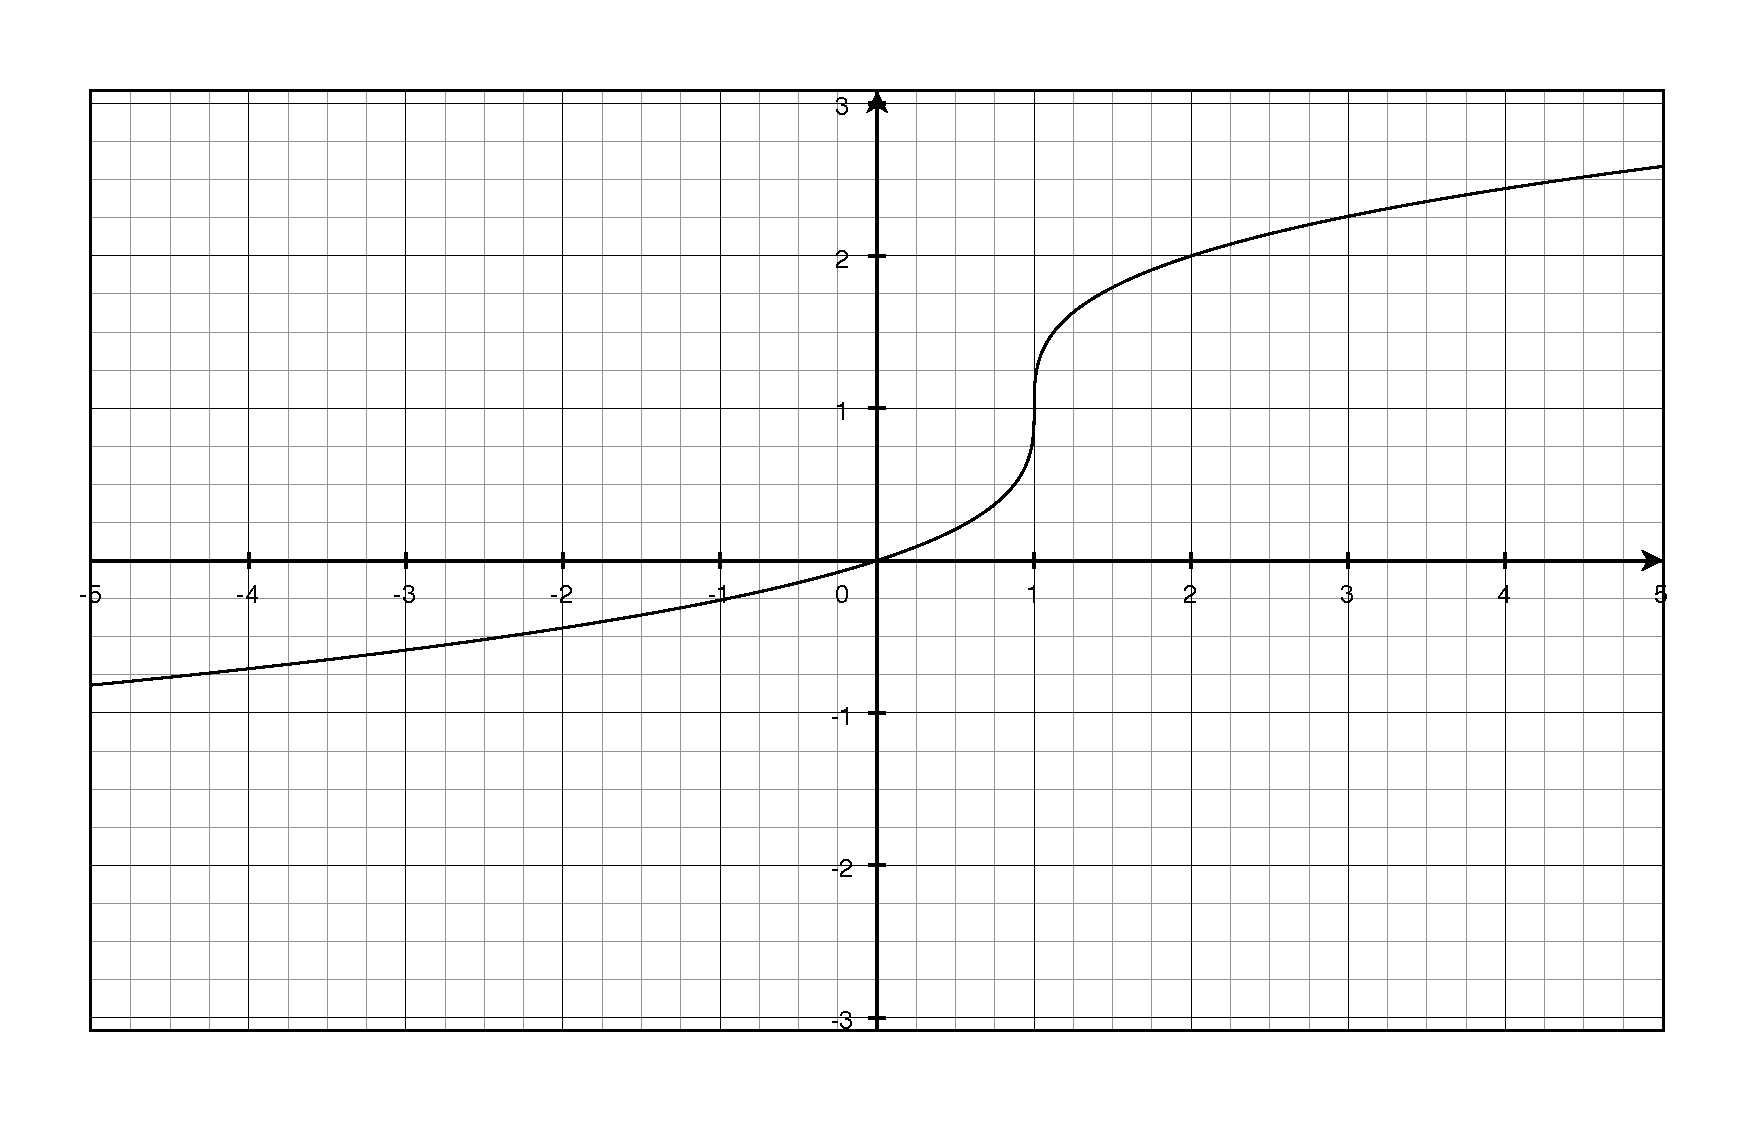
\includegraphics[scale=.3]{question7.eps}
%   \caption*{Question 7}
% \end{figure}

% \begin{tabular}{cc}
% \toprule
% period & amplitude \\
% \midrule
%   $\pi$ & $2$ \\
% \bottomrule
% \end{tabular}

\printanswers

\ifprintanswers 
\usepackage{2in1, lscape} 
\fi

\title{Math 263B \\ Homework Ten}
\date{September 27, 2012}

\begin{document}

\maketitle

\section{Homework}

\begin{itemize*}
  \item Read Section 7.1
  \item pp 310-312: 3-11, 15-22, 27-28
\end{itemize*}

%% \ifprintanswers
%% \pagebreak
%% \fi

\section{Extra Credit}
page 352, problem 43
\ifprintanswers
\begin{solution}
\begin{align*}
  \lim_{n \to \infty} \sum_{i = 1}^n \frac{1}{1 + i/n} \cdot \frac{1}{n} &= \int_1^2 \frac{1}{x} \, \mathrm{d}x \\
  &= \ln x \bigg|_1^2 \\
  &= \ln 2 - \ln 1 \\
  &= \ln 2 \\
\end{align*}
\end{solution}

\section{Section 7.1}

\begin{description}
\item[3]
\[
  D_x \ln(x^2 + 3x + \pi) = \frac{2x + 3}{x^2 + 3x + \pi}
\]

\item[4]
\[
  D_x \ln(3x^3 + 2x) = \frac{9x^2 + 2}{3x^3 + 2x}
\]

\item[5]
\[
  D_x \ln(x - 4)^3 = 3 \cdot D_x \ln(x - 4) = \frac{3}{x - 4}
\]

\item[6]
\[
  D_x \ln (3x - 1)^{1/2} = \frac{1}{2} D_x \ln(3x - 2) = \frac{3}{6x - 4}
\]

\item[7]
\begin{align*}
  y &= 3 \ln x \\
  y' &= \frac{3}{x} \\
\end{align*}

\item[8]
\begin{align*}
  y &= x^2 \ln x \\
  y' &= x + 2x \ln x \\
\end{align*}

\item[9]
\begin{align*}
  z &= x^2 \ln x^2 + (\ln x)^3 \\
    &= 2 x^2 \ln x + (\ln x)^3\\
  z' &= 2x + 4x \ln x + \frac{3 (\ln x)^2}{x} \\
\end{align*}

\item[10]
\begin{align*}
  r &= \frac{\ln x}{x^2 \ln x^2} + \left( \ln x \right)^3 \\
    &= \frac{1}{2x^2} - (\ln x)^3 \\
\\
  \frac{dr}{dx} &= -\frac{1}{x^3} + \frac{3 (\ln x)^2}{x} \\
\end{align*}

\item[11]
\begin{align*}
  g(x) &= \ln ( x + \sqrt{x^2 + 1} ) \\
  g'(x) &= \left( \frac{1}{x + \sqrt{x^2 + 1}} \right) \left(1 + \frac{x}{\sqrt{x^2 + 1}} \right) \\
        &= \frac{1}{\sqrt{x^2 + 1}}
\end{align*}

%% \item[12]
%% \begin{align*}
%%   g(x) &= \ln ( x + \sqrt{x^2 - 1} ) \\
%%   g'(x) &= \left( \frac{1}{x + \sqrt{x^2 - 1}} \right) \left(1 + \frac{x}{\sqrt{x^2 - 1}} \right) \\
%%         &= \frac{1}{\sqrt{x^2 - 1}}
%% \end{align*}

%% \item[13]
%% \begin{align*}
%%   f(x) &= \ln x^{1/3} \\
%%        &= \frac{1}{3} \ln x \\
%%   f'(x) &= \frac{1}{3x} \\
%%   f'(81) &= \frac{1}{243} \\
%% \end{align*}

\item[15]
\begin{align*}
  u &= 2x + 1 \\
  du &= 2 \, dx \\
\\
  \int \frac{1}{2x + 1} \, \mathrm{d}x &= \frac{1}{2} \int \frac{1}{u} \, \mathrm{d}u \\
  &= \frac{1}{2} \ln |u| + C \\
  &= \frac{1}{2} \ln | 2x + 1 | + C \\
\end{align*}

\item[16]
\begin{align*}
  u &= 1 - 2x \\
  du &= - 2 \, dx \\
\\
  \int \frac{1}{1 - 2x} \, \mathrm{d}x &= - \frac{1}{2} \int \frac{1}{u} \, \mathrm{d}u \\
  &= - \frac{1}{2} \ln |u| + C \\
  &= - \frac{1}{2} \ln | 1 - 2x | + C \\
\end{align*}


\item[17]
\begin{align*}
  u &= 3v^2 + 9v \\
  du &= (6v + 9) \, dv \\
\\
  \int \frac{6v + 9}{3v^2 + 9v} \, \mathrm{d}v &= \int \frac{1}{u} \, \mathrm{d}u \\
  &= \ln |u| + C \\
  &= \ln | 3v^2 + 9v | + C \\
\end{align*}

\item[18]
\begin{align*}
  u &= 2x^2 + 8 \\
  du &= 4x \, dx \\
\\
  \int \frac{x}{2x^2 + 8} \, \mathrm{d}v &= \frac{1}{4} \int \frac{1}{u} \, \mathrm{d}u \\
  &= \frac{1}{4} \ln |u| + C \\
  &= \frac{1}{4} \ln | 2x^2 + 8 | + C \\
\end{align*}

\item[19]
\begin{align*}
  u &= \ln x \\
  du &= \frac{1}{x} \, dx \\
\\
  \int \frac{2 \ln x}{x} \, \mathrm{d}x &= 2 \int u \, \mathrm{d}u \\
  &= u^2 + C \\
  &= (\ln x)^2 + C \\
\end{align*}

\item[20]
\begin{align*}
  u &= - \frac{1}{\ln x} \\
  du &= - \frac{1}{x (\ln x)^2} \, dx \\
\\
  \int \frac{-1}{x (\ln x)^2} \, \mathrm{d}x &= \int \, \mathrm{d}u \\
  &= u + C \\
  &= - \frac{1}{\ln x} + C \\
\end{align*}

\item[21]
\begin{align*}
  u &= 2x^5 + \pi \\
  du &= 10x^4 \, dx \\
  u(0) &= \pi \\
  u(3) &= 486 + \pi \\
\\
  \int_0^3 \frac{x^4}{2x^5 + \pi} \, \mathrm{d}x &= \frac{1}{10} \int_{\pi}^{486 + \pi} \frac{1}{u} \, \mathrm{d}u \\
  &= \frac{1}{10} \ln u \bigg|_{\pi}^{486 + \pi} \\
  &= \frac{1}{10} [ \ln(486 + \pi) - \ln(\pi) ] \\
  &\approx 0.50479 \\
\end{align*}

\item[22]
\begin{align*}
  u &= 2t^2 + 4t + 3 \\
  du &= 4(t + 1) \, dt \\
  u(0) &= 3 \\
  u(1) &= 9 \\
\\
  \int_0^1 \frac{t + 1}{2t^2 + 4t + 3} \, \mathrm{d}t &= \frac{1}{4} \int_3^9 \frac{1}{u} \, \mathrm{d}u \\
  &= \frac{1}{4} \ln u \bigg|_3^9 \\
  &= \frac{1}{4} [ \ln 9 - \ln 3 ] \\
  &\approx 0.27465 \\
\end{align*}

\item[27]
\begin{align*}
  y &= \frac{x + 11}{\sqrt{x^3 - 4}} \\
  \ln y &= \ln(x + 11) - \frac{1}{2} \ln(x^3 - 4) \\
\\
  y' \cdot \frac{1}{y} &= \frac{1}{x + 11} - \frac{3x^2}{2(x^3 - 4)} \\
  &= \frac{-x^3 - 33x^2 - 8}{2(x + 11)(x^3 - 4)} \\
\\
  y' &= \frac{-x^3 - 33x^2 - 8}{2(x^3 - 4)^{3/2}}
\end{align*}

\item[28]
\begin{align*}
  y &= (x^2 + 3x)(x-2)(x^2+1) \\
  \ln y &= \ln(x^2 + 3x) + \ln(x-2) + \ln(x^2 + 1) \\
\\
  y' \cdot \frac{1}{y} &= \frac{2x + 3}{x^2 + 3x} + \frac{1}{x-2} + \frac{2x}{x^2 + 1} \\
\\
  y' &= 5x^4 + 4x^3 - 15x^2 + 3x - 6 \\
\end{align*}

\end{description}

\else

\vspace{8 cm}
{\em Wherever we are, what we hear is mostly noise. When we ignore it, it disturbs us.  When we listen to it, we find it fascinating.}

\hspace{0.5 cm} --John Cage

%% {\em Some writers have so confounded society with government, as to leave little or no distinction between them; whereas
%%   they are not only different, but have different origins. Society is produced by our wants, and government by our
%%   wickedness; the former promotes our happiness POSITIVELY by uniting our affections, the latter NEGATIVELY by
%%   restraining our vices. The one encourages intercourse, the other creates distinctions. The first a patron, the last a
%%   punisher.} --Thomas Paine

%% Value judgments are destructive to our proper business, which is curiosity and awareness. -- John Cage
\fi

\end{document}

